\section{Simplified Environment Results}

All three algorithms successfully converge to a decent grasping policy in the simplified environment. BDQ and DQN  were trained with varying action dimension padding 2, 4, 8, 16, and 33.
We observed how the neural network size affects the success rate. Two different network sizes were tried xon BDQ; a large network with two hidden layers in the shared module with 512 and 256 neurons each and 128 each for state and advantage function estimators, and a small network with two hidden layers in the shared representation with 64 neurons each and 32 neurons each for the state and advantage function estimators. Furthermore, we compared the BDQ performance with two different buffer sizes, fifty thousand and one million. We did not vary the DQN algorithm's hyperparameters. The default buffer size of fifty thousand was used for all trials of DQN.
As for the SAC algorithm, we only change the input from the encoder to depth in the simplified environment.

All BDQ trials converged the same success rate during training except the big network variant \ref{fig:bdqincrease}. BDQ with four pads achieved the best test success rate in the floor environment, with 94\%. BDQ with 16pads came second with a 93\% success rate. However, they switched sides in the table scene, where BDQ 16pads achieved 91\%, BDQ 4 pads stuck at an 89\% success rate. We noticed the significant performance difference between the big neural network and the small one in the figure \ref{fig:BDQnetwork}. The small network achieves far more notable results, where the big network failed to learn the simplified environment.

DQN algorithm succeeded in learning the simplified environment. However, its top performance lagged significantly behind the BDQ algorithm with a 74\% success in the floor scene and a 63\% success in table scene. We observed the deteriorated results with an increase in action space dimension. The results are depicted in the figure \ref{fig:dqnincrease}.

SAC algorithm achieved the best training results converged to the highest success rate. It achieved a 97\% success rate in the floor scene and an 87\% success rate in the table scene. Interestingly, BDQ 16pads surpassed SAC's performance with a 91\% success in the table scene. However, as shown in figure \ref{fig:sacvsbdq}, SAC converged to a higher success rate than the BDQ during training.

\begin{table}[!htbp]
    \begin{tabular}{l|l|l|l|l|}
    \cline{2-5}
                       & \multicolumn{4}{c|}{\textbf{BDQ Simplified Scenario}}              \\ \cline{2-5}
                       & \multicolumn{2}{c|}{\textbf{Floor Scene}} & \multicolumn{2}{c|}{\textbf{Table Scene}} \\ \hline
    \multicolumn{1}{|l|}{\textbf{Models}}    & \multicolumn{1}{c|}{\textbf{\begin{tabular}[c]{@{}c@{}}Training Set\\ (\%)\end{tabular}}} & \multicolumn{1}{c|}{\textbf{\begin{tabular}[c]{@{}c@{}}Test Set\\ (\%)\end{tabular}}} & \multicolumn{1}{c|}{\textbf{\begin{tabular}[c]{@{}c@{}}Training Set\\ (\%)\end{tabular}}} & \multicolumn{1}{c|}{\textbf{\begin{tabular}[c]{@{}c@{}}Test Set\\ (\%)\end{tabular}}} \\ \hline
    \multicolumn{1}{|l|}{\textbf{BDQ\_33pads\_big}}   & 34              & 29         & 13              & 12         \\ \hline
    \multicolumn{1}{|l|}{\textbf{BDQ\_33pads\_small}} & 90              & 82         & 86              & 79         \\ \hline
    \multicolumn{1}{|l|}{\textbf{BDQ\_16pads\_small}} & 89              & 93         & 90              & 91         \\ \hline
    \multicolumn{1}{|l|}{\textbf{BDQ\_8pads\_small}}  & 91              & 90         & 77              & 72         \\ \hline
    \multicolumn{1}{|l|}{\textbf{BDQ\_4\_pads}}       & 96              & 94         & 92              & 89         \\ \hline
    \end{tabular}
    \caption{BDQ algorithm's result in the simplified environment \label{tab:BDQsimpres}}
\end{table}


\begin{table}[!htbp]
    \begin{tabular}{l|l|l|l|l|}
    % \hline
    \cline{2-5}
                         & \multicolumn{4}{c|}{\textbf{DQN Simplified Scenario}}                                 \\ \cline{2-5}
                         & \multicolumn{2}{c|}{\textbf{Floor Scene}} & \multicolumn{2}{c|}{\textbf{Table Scene}} \\ \hline
    \multicolumn{1}{|l|}{\textbf{Models}}     & \multicolumn{1}{c|}{\textbf{\begin{tabular}[c]{@{}c@{}}Training Set\\ (\%)\end{tabular}}} & \multicolumn{1}{c|}{\textbf{\begin{tabular}[c]{@{}c@{}}Test Set\\ (\%)\end{tabular}}} & \multicolumn{1}{c|}{\textbf{\begin{tabular}[c]{@{}c@{}}Training Set\\ (\%)\end{tabular}}} & \multicolumn{1}{c|}{\textbf{\begin{tabular}[c]{@{}c@{}}Test Set\\ (\%)\end{tabular}}} \\ \hline
    \multicolumn{1}{|l|}{\textbf{DQN\_33pads}} & 6                  & 6              & 6                  & 7              \\ \hline
    \multicolumn{1}{|l|}{\textbf{DQN\_16pads}} & 12                 & 6              & 9                  & 14             \\ \hline
    \multicolumn{1}{|l|}{\textbf{DQN\_8pads}}  & 75                 & 65             & 38                 & 40             \\ \hline
    \multicolumn{1}{|l|}{\textbf{DQN\_4pads}}  & 75                 & 73             & 1                  & 1              \\ \hline
    \multicolumn{1}{|l|}{\textbf{DQN\_2pads}}  & 76                 & 74             & 55                 & 63             \\ \hline
    \end{tabular}
    \caption{DQN algorithm's result in the simplified environment}
\end{table}



\begin{table}[!htbp]
    \begin{tabular}{l|l|l|l|l|}
    \cline{2-5}
                                    & \multicolumn{4}{c|}{\textbf{SAC Simplified  Scenario}}                         \\ \cline{2-5}
                                    & \multicolumn{2}{c|}{\textbf{Floor Scene}} & \multicolumn{2}{c|}{\textbf{Table Scene}} \\ \hline
    \multicolumn{1}{|l|}{\textbf{Models}}    & \multicolumn{1}{c|}{\textbf{\begin{tabular}[c]{@{}c@{}}Training Set\\ (\%)\end{tabular}}} & \multicolumn{1}{c|}{\textbf{\begin{tabular}[c]{@{}c@{}}Test Set\\ (\%)\end{tabular}}} & \multicolumn{1}{c|}{\textbf{\begin{tabular}[c]{@{}c@{}}Training Set\\ (\%)\end{tabular}}} & \multicolumn{1}{c|}{\textbf{\begin{tabular}[c]{@{}c@{}}Test Set\\ (\%)\end{tabular}}} \\ \hline
    \multicolumn{1}{|l|}{\textbf{SAC\_encoder}} & 98                & 97              & 84                 & 87             \\ \hline
    \multicolumn{1}{|l|}{\textbf{SAC\_depth}}   & 91                & 96              & 28                 & 24             \\ \hline
    \end{tabular}
    \caption{SAC algorithm's result in the simplified environment}
\end{table}

\begin{figure}[!htbp]
    \begin{subfigure}{0.49\textwidth}
        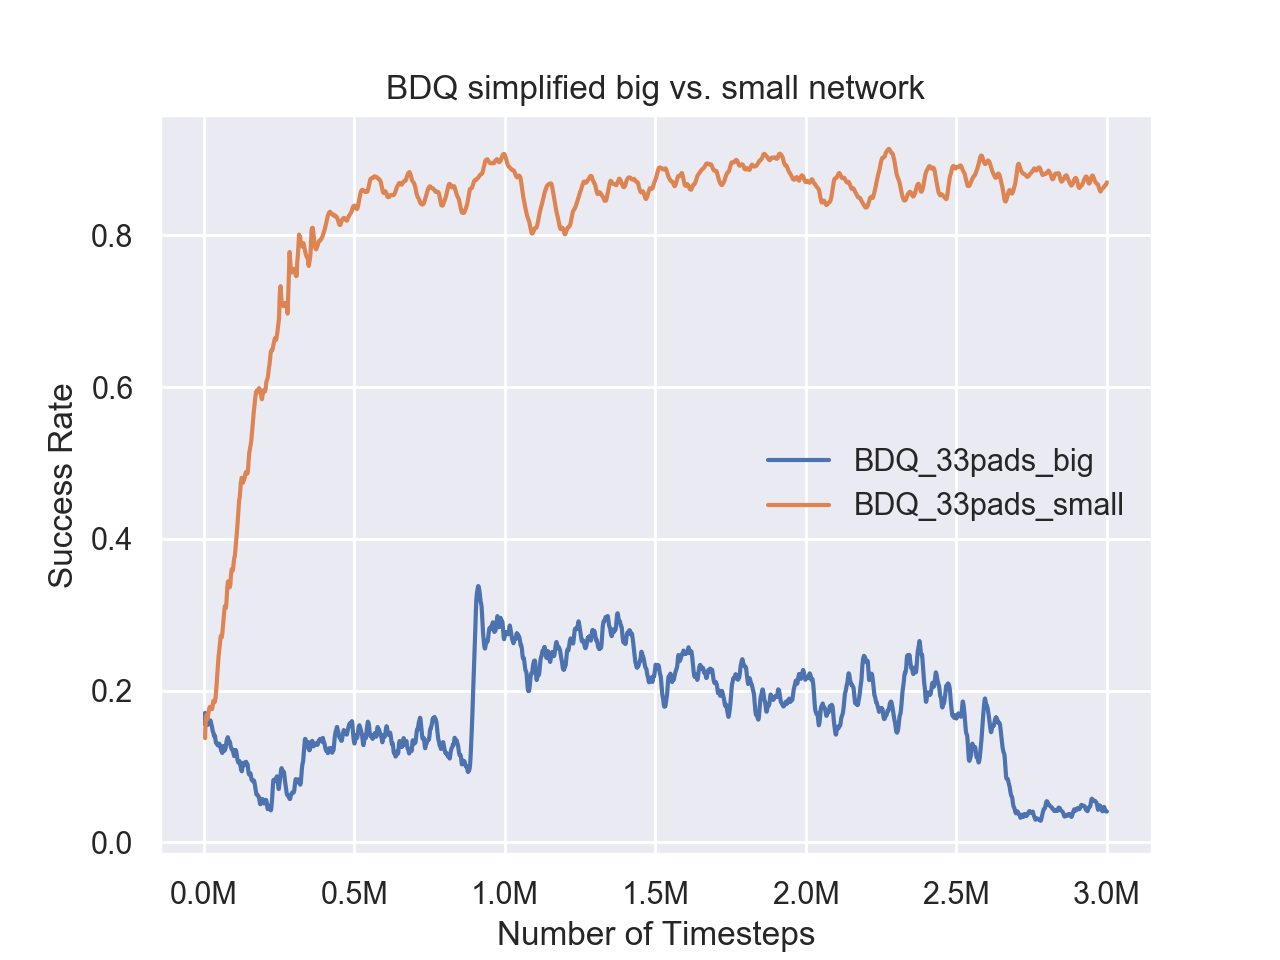
\includegraphics[width=\linewidth]{figures/BDQ_simplified_big_vs_small_network_no_var}
        \caption{BDQ performance with big and small network size} \label{fig:BDQnetwork}
    \end{subfigure}%
    \hspace*{\fill}   % maximize separation between the subfigures
    \begin{subfigure}{0.49\textwidth}
        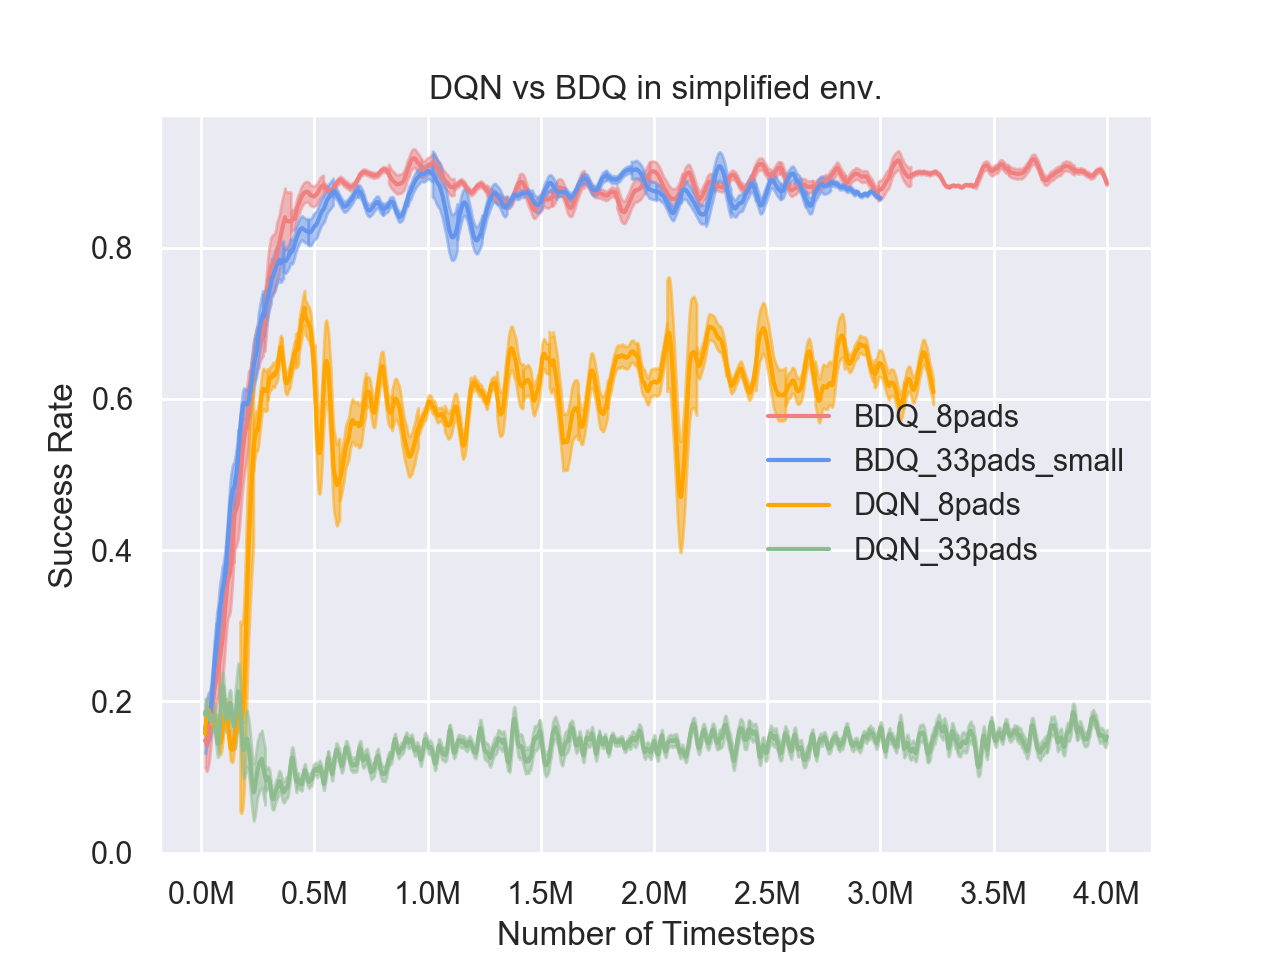
\includegraphics[width=\linewidth]{figures/DQN_vs_BDQ_in_simplified_env}
        \caption{BDQ vs DQN performance with increasing action space. Shaded area shows the standard deviation} \label{fig:BDQDQNsimp}
    \end{subfigure}%
    \hspace*{\fill}   % maximize separation between the subfigures
\caption{ BDQ network size comparison and its performance against DQN with increasing action space dimension in simplified environment\label{fig:BDQDQN}}
\end{figure}

\begin{figure}[!htbp]
    \begin{subfigure}{0.49\textwidth}
        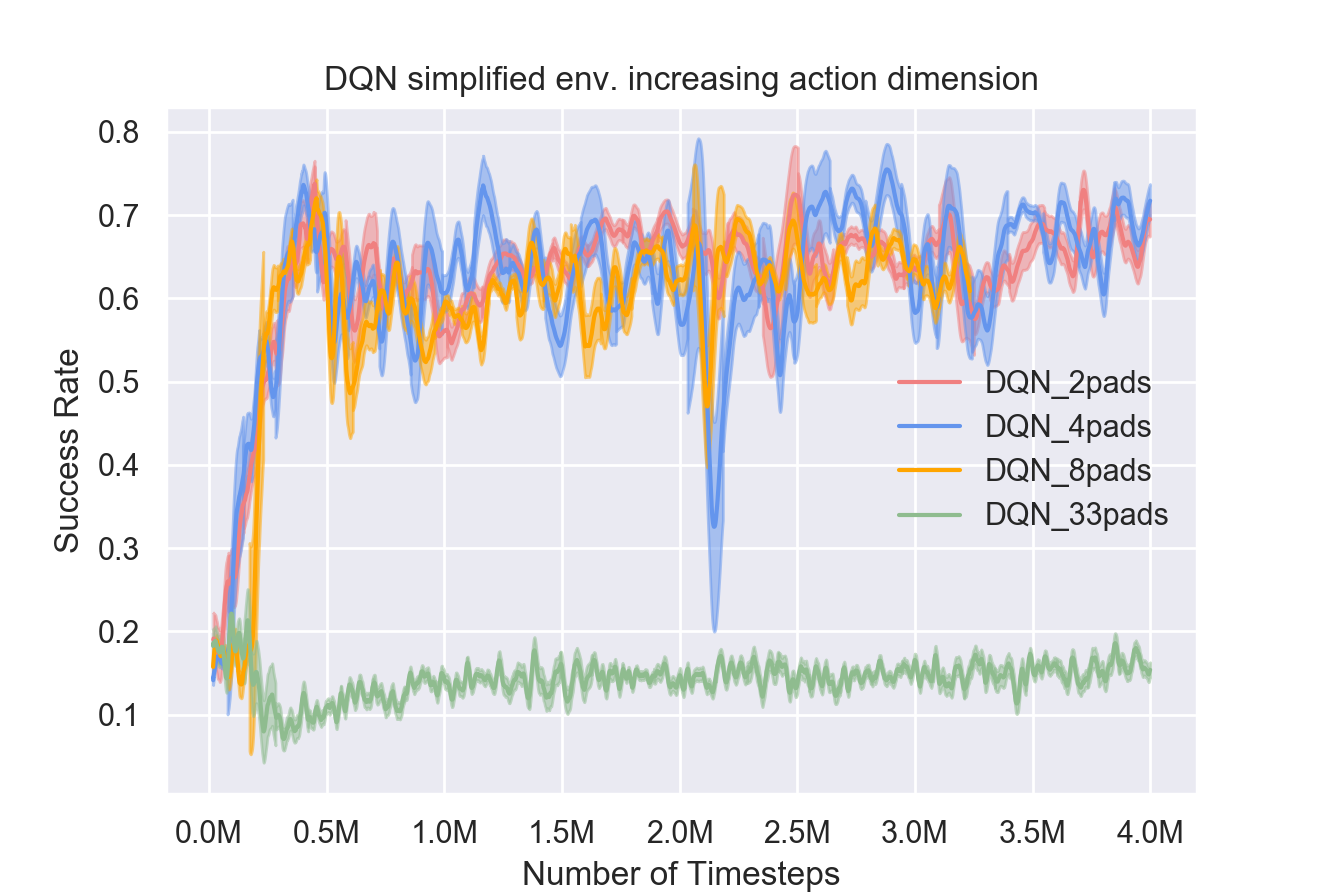
\includegraphics[width=\linewidth]{figures/DQN_simplified_env_increasing_action_dimension}
        \caption{DQN performance with increasing action space dimenstion.} \label{fig:dqnincrease}
    \end{subfigure}%
    \hspace*{\fill}   % maximize separation between the subfigures
    \begin{subfigure}{0.49\textwidth}
        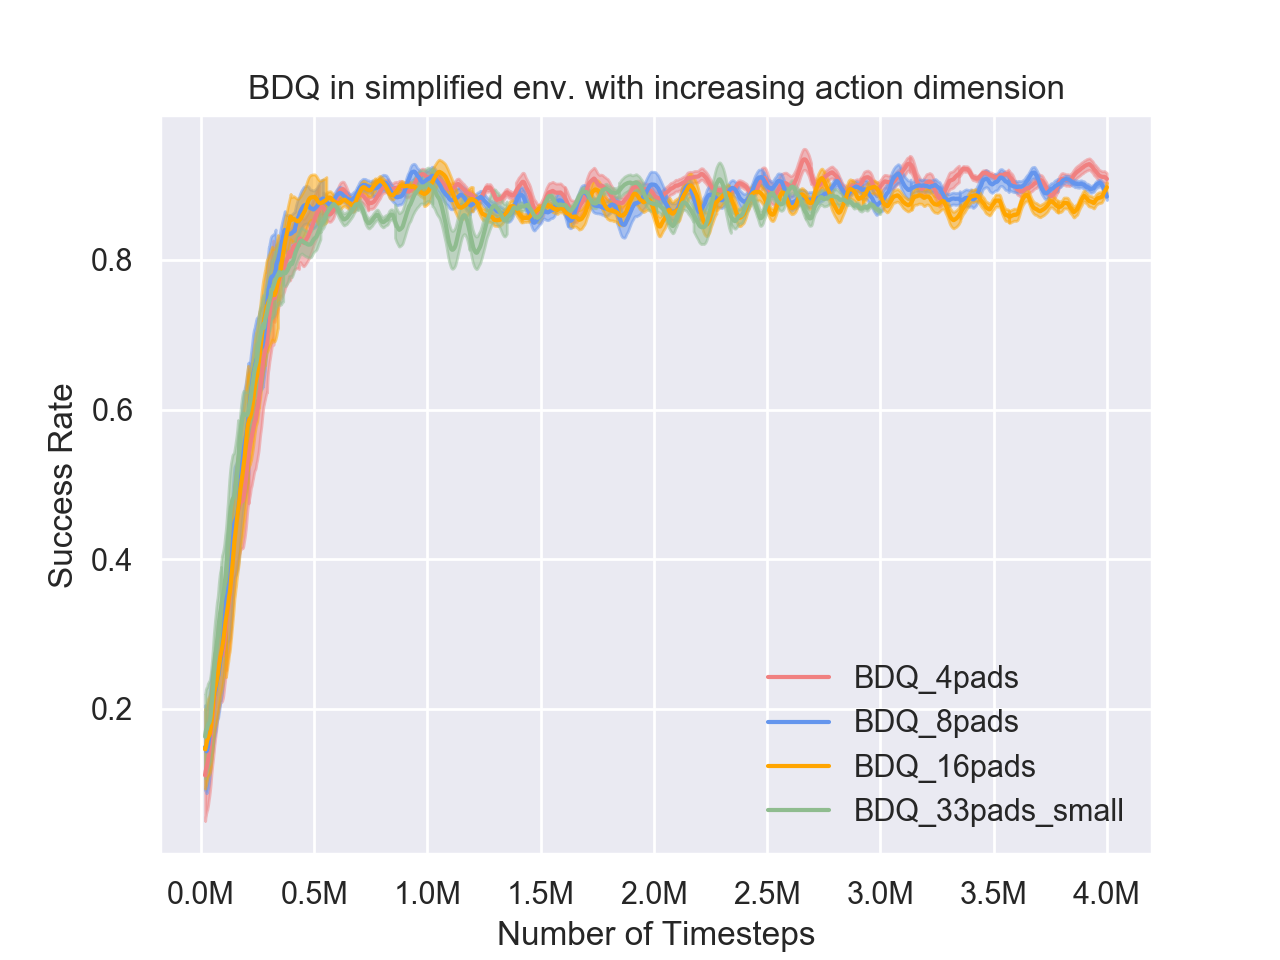
\includegraphics[width=\linewidth]{figures/BDQ_in_simplified_env_with_increasing_action_dimension}
        \caption{BDQ performance with increasing action space dimenstion.} \label{fig:bdqincrease}
    \end{subfigure}%
    \hspace*{\fill}   % maximize separation between the subfigures


\caption{BDQ and DQN performances in simplified environment with increasing action space dimension. Shaded areas show the standard deviation \label{fig:scenes}}
\end{figure}



\begin{figure}[!htbp]
    \begin{subfigure}{0.49\textwidth}
        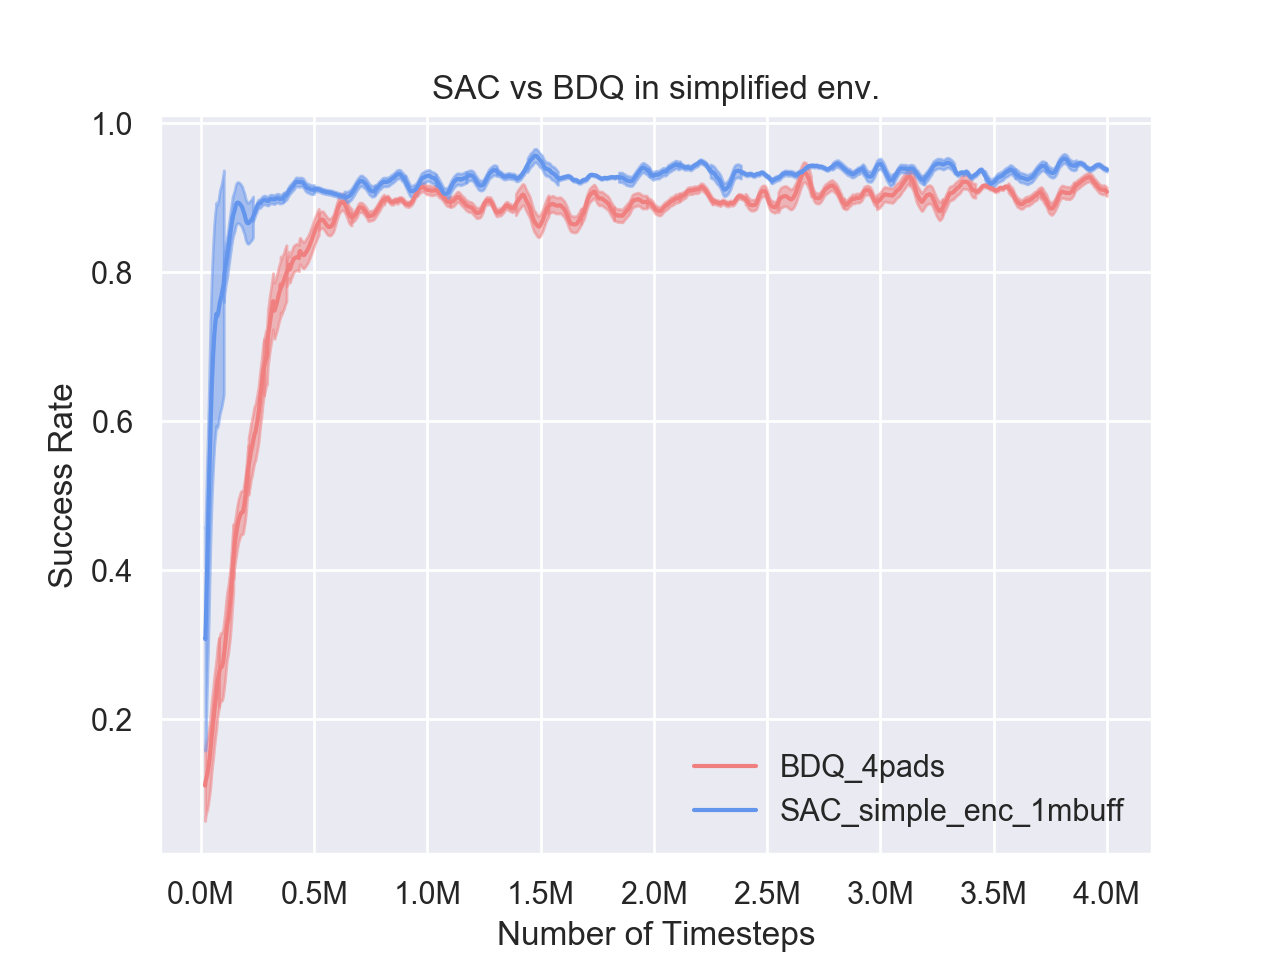
\includegraphics[width=\linewidth]{figures/SAC_vs_BDQ_in_simplified_env}
        \caption{Best BDQ model compared to the best SAC model in simplified environment} \label{fig:sacvsbdq}
    \end{subfigure}%
    \hspace*{\fill}   % maximize separation between the subfigures
    \begin{subfigure}{0.49\textwidth}
        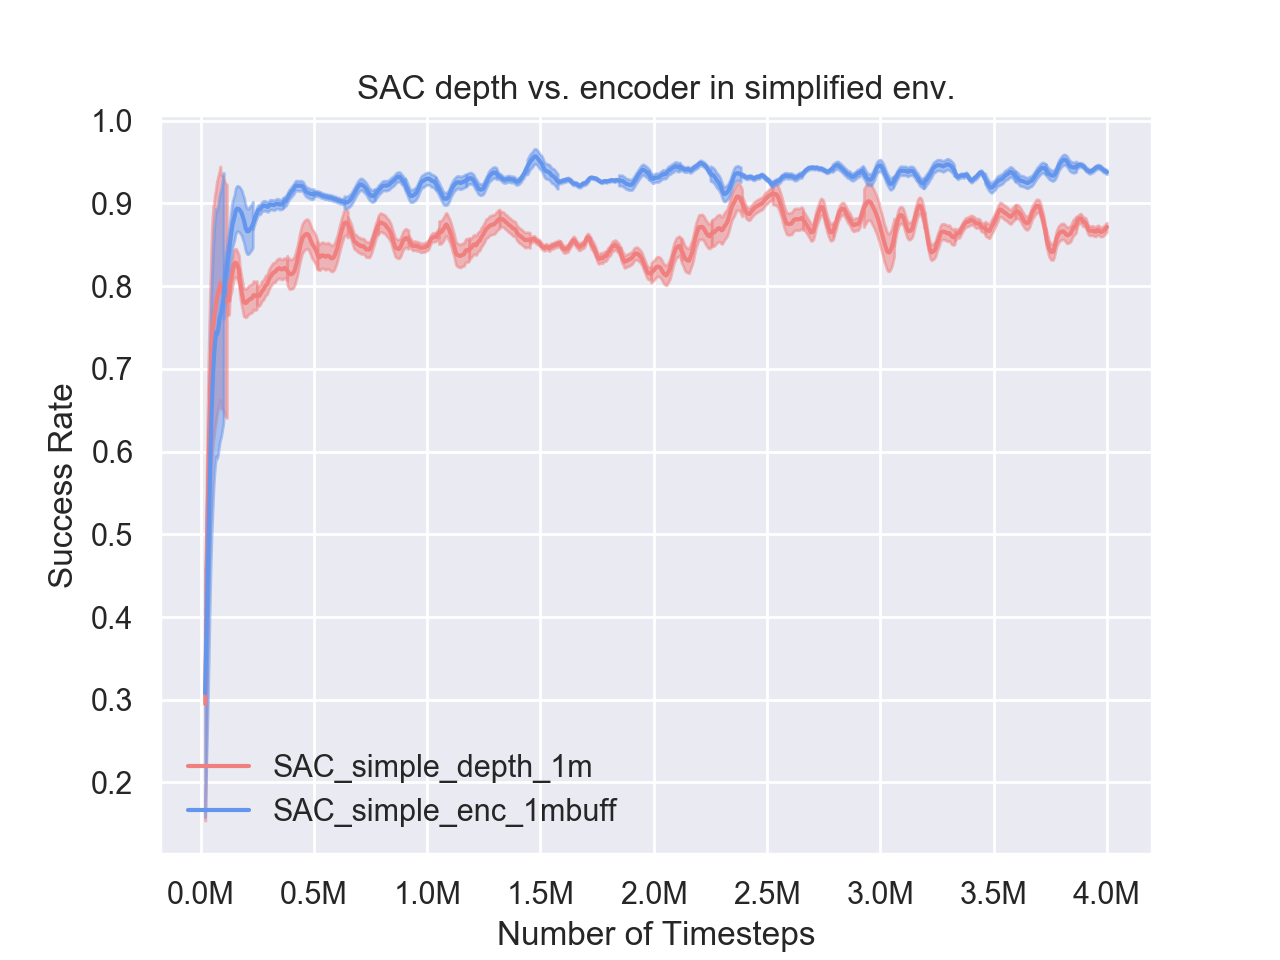
\includegraphics[width=\linewidth]{figures/SAC_depth_vs_encoder_in_simplified_env}
        \caption{SAC depth compared to encoder perception in simplified environment} \label{fig:floor}
    \end{subfigure}%
    \hspace*{\fill}   % maximize separation between the subfigures


\caption{ SAC results in simplified environment\label{fig:scenes}}
\end{figure}

% \begin{figure}[!htbp]
%     \centering
%         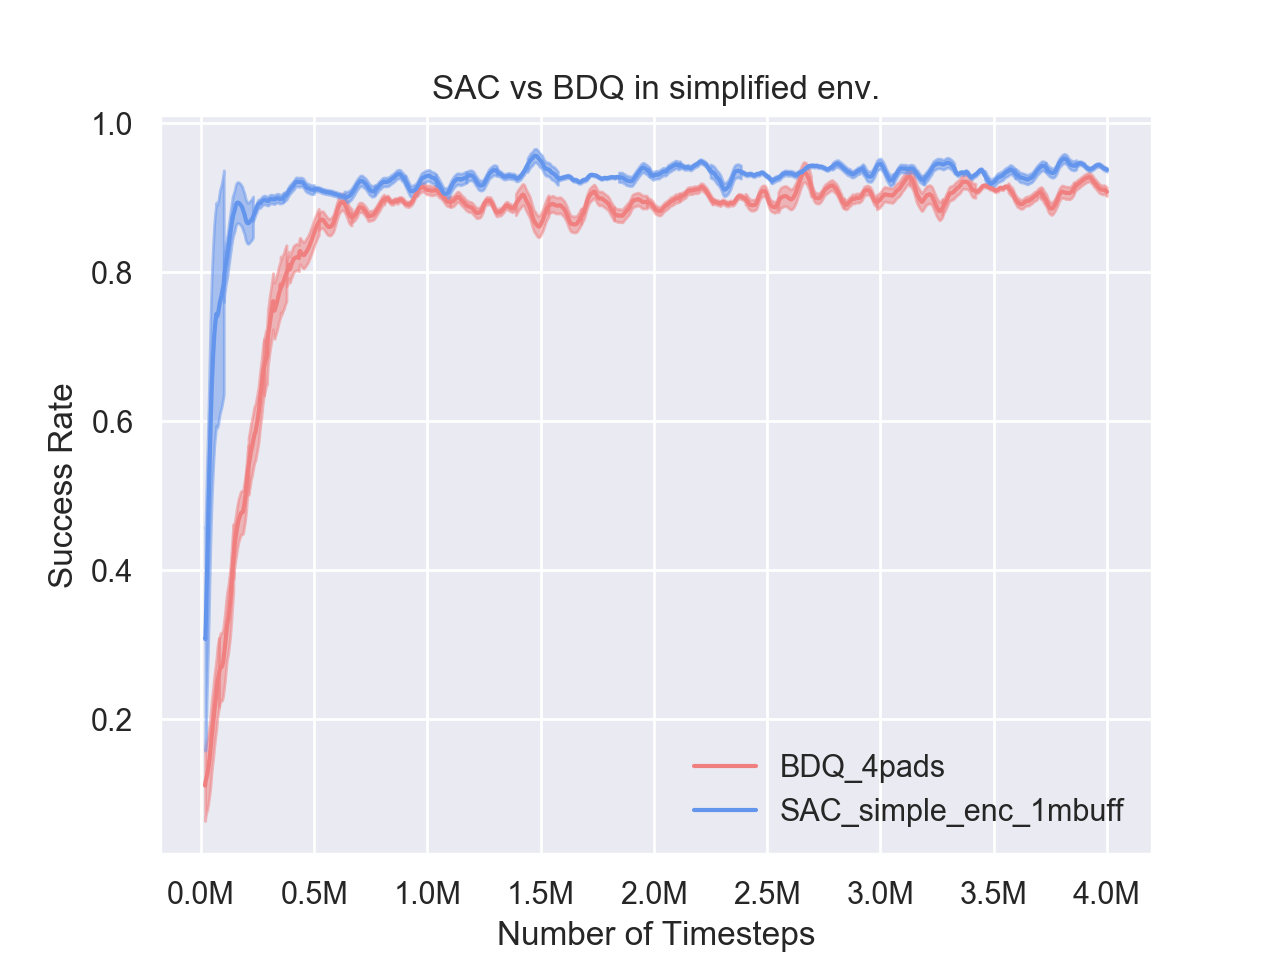
\includegraphics[width=0.4\textwidth]{figures/SAC_vs_BDQ_in_simplified_env}
%     \caption{Different manipulation skill adopted to robotic manipulators \cite{Kroemer2019}}
%     \label{fig:x manipulation_skills}
% \end{figure}

% \begin{figure}[!htbp]
%     \centering
%         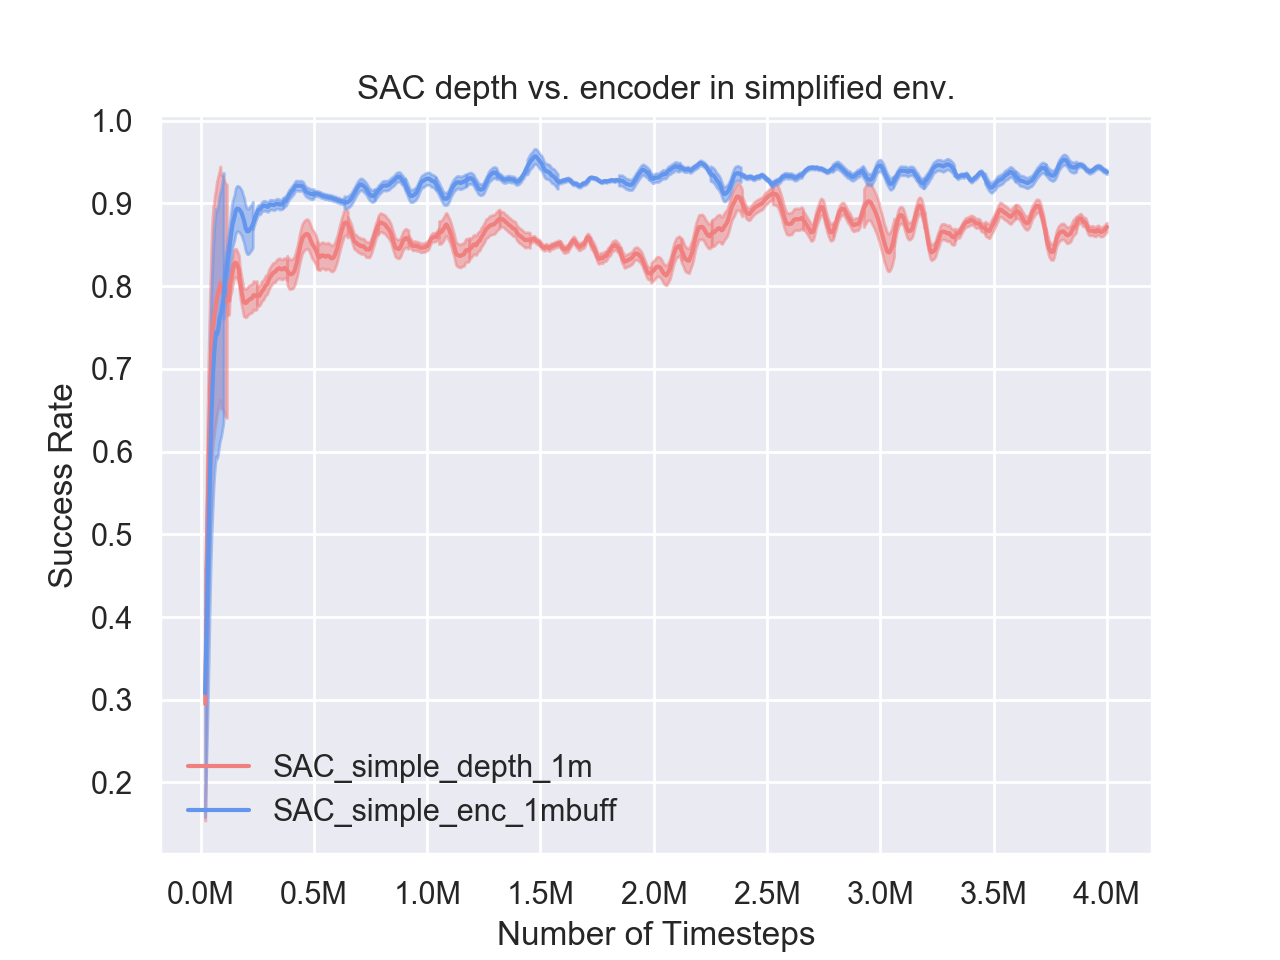
\includegraphics[width=0.4\textwidth]{figures/SAC_depth_vs_encoder_in_simplified_env}
%     \caption{Different manipulation skill adopted to robotic manipulators \cite{Kroemer2019}}
%     \label{fig:x manipulation_skills}
% \end{figure}

